
\subsection{Herramienta Utilizadas} 
    

\subsubsection*{Kali Linux}
Kali Linux es una distribución de Linux (basada en Debian) centrada en la seguridad. 
Es una versión renombrada de la famosa distribución de Linux conocida como Backtrack, 
que venía con un enorme repositorio de herramientas de piratería de código abierto, 
para pruebas de penetración de aplicaciones \emph{web}, inalámbricas y de red. 

\begin{center}
    \begin{figure}   
       \begin{center}
          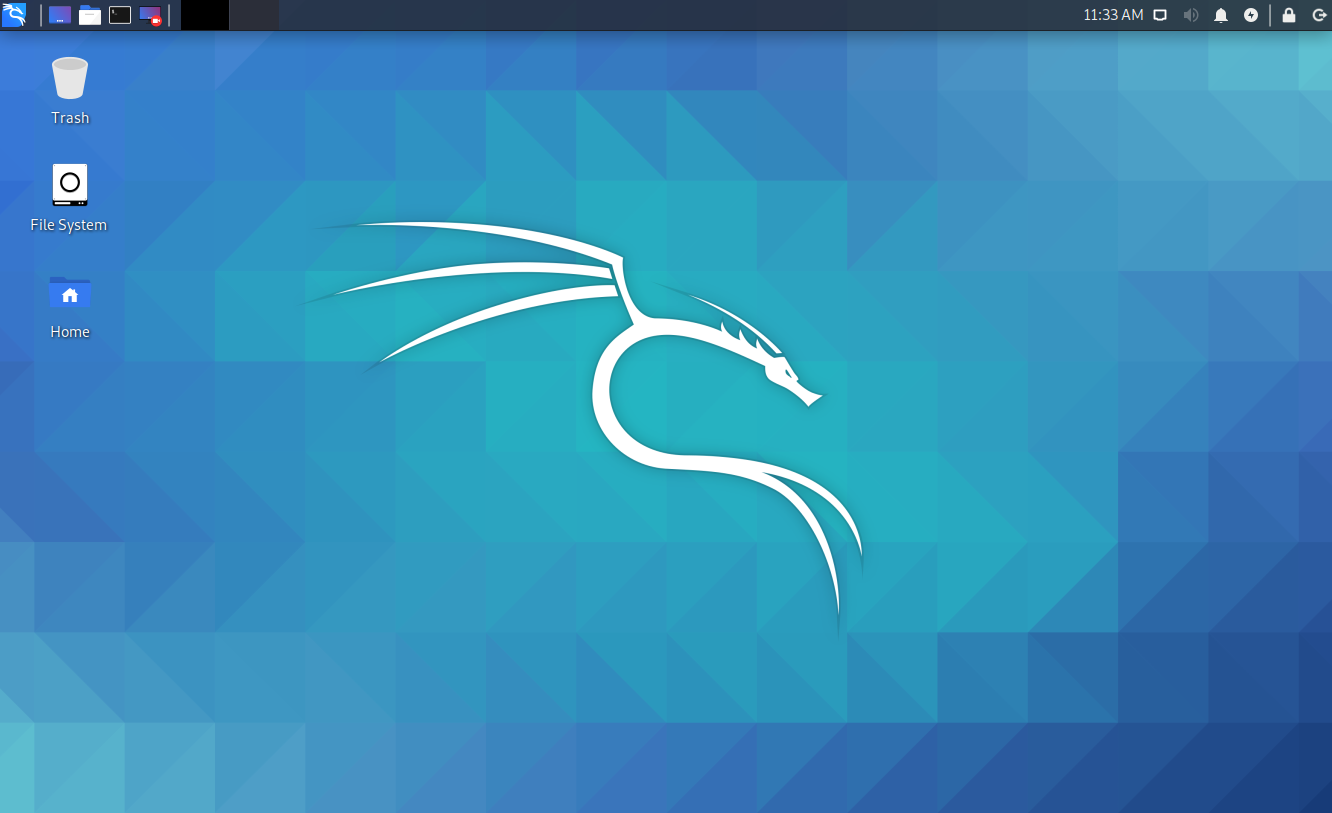
\includegraphics[width=11cm,height=7cm]{ataque-1.png}
       \end{center}
       \caption{Escritorio de Kali Linux}
    \end{figure}
 \end{center}
 

Kali Linux contiene muchas herramientas preinstaladas con 
todas las dependencias y ya está lista para usar. Esto nos permite tener que prestar 
más atención a las pruebas y no a la instalación de la herramienta. Las actualizaciones 
para las herramientas instaladas en Kali Linux se publican con mayor frecuencia, 
lo que le ayuda a mantener las a las mismas actualizadas.

Esta distribución contiene las herramientas necesarias para realizar nuestro
ataque.

\subsubsection*{Wireshark}
Wireshark es uno de los analizadores de protocolos de red más populares, es de 
código abierto y gratuito. Wireshark está preinstalado en Kali y es ideal para la 
resolución de problemas de red, análisis y, para este caso de estudio, una herramienta 
perfecta para monitorear el tráfico de posibles objetivos. Wireshark usa un kit de 
herramientas para implementar su interfaz de usuario y para capturar paquetes. 
Funciona de manera muy similar a un comando \emph{tcpdump}; sin embargo, nos brinda
una interfaz gráfica, posee opciones integradas de clasificación y filtrado.

\begin{center}
    \begin{figure}   
       \begin{center}
          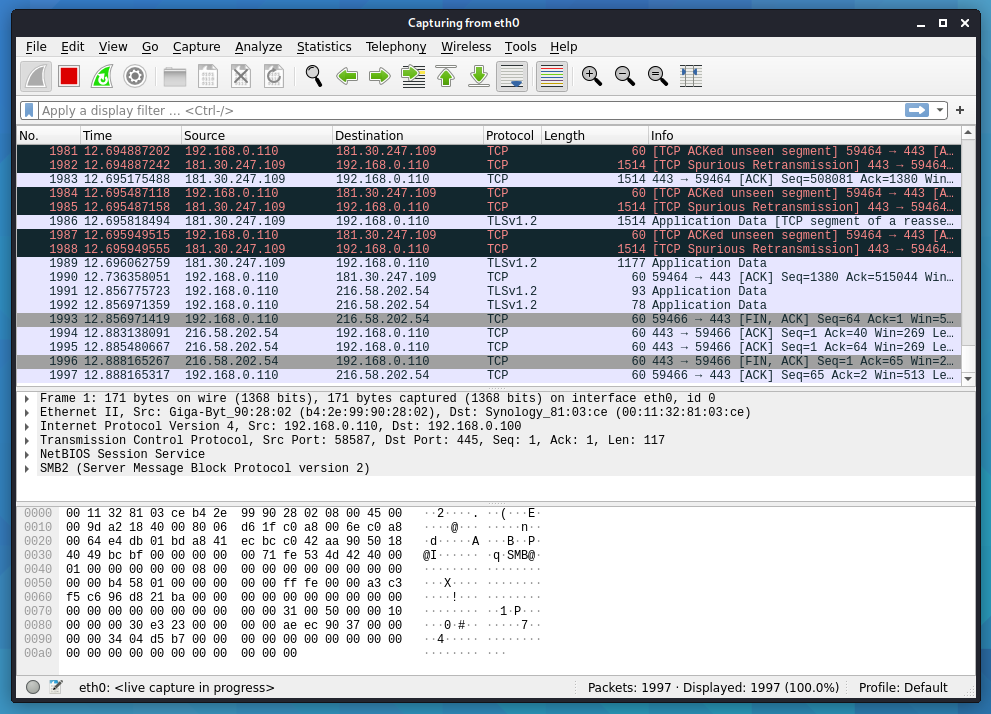
\includegraphics[width=10cm,height=7cm]{wireshark.png}
       \end{center}
       \caption{Interface del Wireshark}
    \end{figure}
 \end{center}
 
\subsubsection*{Ettercap}

\begin{center}
   \begin{figure}   
      \begin{center}
         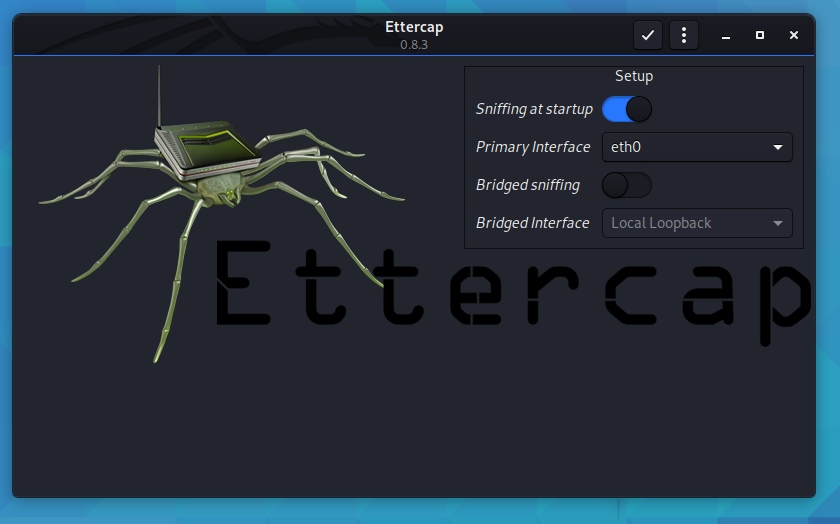
\includegraphics[width=10 cm,height=7cm]{ataque-2.png}
      \end{center}
      \caption{Ettercap}
   \end{figure}
\end{center}

Ettercap es un paquete completo gratuito y de código abierto para ataques basados 
en intermediarios. Ettercap se puede utilizar para análisis de protocolos de redes 
informáticas y auditorías de seguridad, con funciones de rastreo de conexiones en 
tiempo real y filtrado de contenido. Ettercap funciona configurando la interfaz de red 
del atacante en modo promiscuo y \emph{ARP} para envenenar las máquinas víctimas.



\subsection{Realización del ataque}

\begin{center}
    \begin{figure}   
       \begin{center}
         
          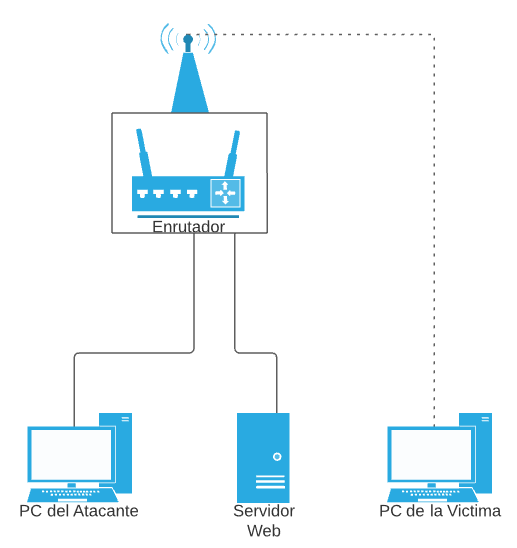
\includegraphics[width=9cm,height=9cm]{red.png}
       \end{center}
       \caption{Escenario montado}
       \label{escMontado}
    \end{figure}
 \end{center}

La idea principal de esta sección es demostrar que, encontrándose en una red interna
y con ciertas herramientas, es posible realizar un ataque 
sin necesidad de conocer a fondo la implementación de la misma ni de tener mayores
privilegios.

El escenario montado (figuras \ref{escMontado} y \ref{formMontado}) consiste en crear una página \emph{web} con un 
formulario donde se debe completar con usuario y contraseña, y un 
submit el cual envía esta información desde el cliente hasta el 
servidor \emph{web}. El envío de este formulario contiene la información confidencial,
 por lo que en un escenario seguro ningún
intermediario podría obtener estos datos. Dado que este tráfico
circula utilizando el protocolo \emph{HTTP}, mostraremos como nos podemos hacer de las credenciales
ingresadas por el usuario.

\begin{center}
   \begin{figure}   
      \begin{center}
         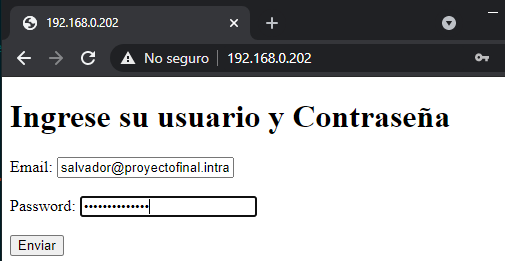
\includegraphics[width=10.5cm,height=6cm]{form.png}
      \end{center}
      \caption{Formulario montado}
      \label{formMontado}
   \end{figure}
\end{center}

\subsection{Preparando Ettercap para el ataque ARP Poisoning}

Lo primero que debemos hacer, en la lista de aplicaciones, es buscar el apartado 
\emph{Sniffing} y \emph{Spoofing}, ya que es allí donde encontraremos las herramientas necesarias
 para llevar a cabo este ataque. A continuación, abriremos Ettercap.



El siguiente paso es seleccionar la tarjeta de red con la que vamos a trabajar. Para 
ello, en el menú superior de Ettercap seleccionaremos \textsc{Sniff} $>$ \textsc{Unified Sniffing} y, 
cuando nos lo pregunte, seleccionaremos nuestra tarjeta de red (por ejemplo, en 
nuestro caso, \textsc{eth0}).

Luego buscaremos todos los hosts conectados a nuestra red local. Para ello, 
seleccionaremos \textsc{Hosts} del menú de la parte superior y seleccionaremos la primera 
opción, Hosts List (Figura \ref{ettercap}).

Allí veremos todos los hosts o dispositivos conectados a nuestra red. 
Sin embargo, en caso de que no estén todos, podemos realizar una exploración 
completa de la red simplemente abriendo el menú \textsc{Hosts} y seleccionando la opción 
\textsc{Scan for hosts}. Tras unos segundos, la lista de antes se debería actualizar 
mostrando todos los dispositivos, con sus respectivas \emph{IPs} y \emph{MACs}, conectados 
a nuestra red.



\subsection{Nuestro Ettercap ya está listo. Ya podemos empezar con el ataque ARP Poisoning}

En caso de querer realizar un ataque dirigido contra un solo host, por ejemplo, 
suplantar la identidad de la puerta de enlace para monitorear las conexiones 
de la víctima, antes de empezar con el 
ataque debemos establecer los dos objetivos.

Para ello, debajo de la lista de hosts podemos ver tres botones, aunque nosotros 
prestaremos atención a los dos últimos:

    Target 1 – Seleccionamos la \emph{IP} del dispositivo a monitorear, en este caso, 
    la computadora de la víctima, y pulsamos sobre dicho botón.

    Target 2 – Pulsamos la \emph{IP} que queremos suplantar, en este caso, la de la 
    puerta de enlace y la del servidor \emph{web}.

    \begin{center}
        \begin{figure}   
           \begin{center}
              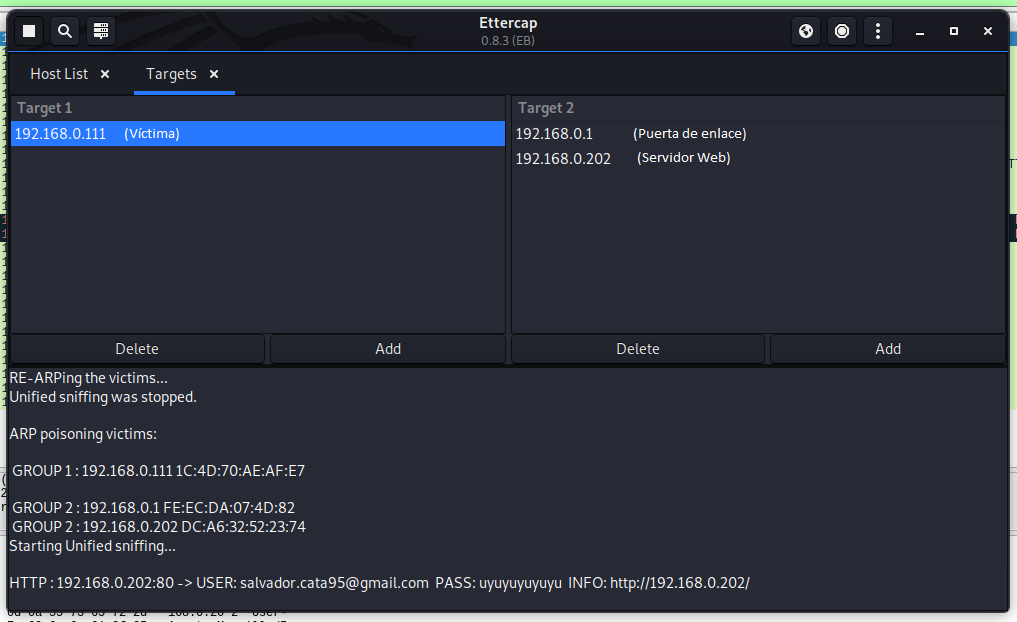
\includegraphics[width=17cm,height=9.5cm]{ataque-7-deta.png}
           \end{center}
           \caption{Ettercap}
           \label{ettercap}
        \end{figure}
     \end{center}

Debemos elegir el menú \textsc{MITM} de la parte superior y, en él, 
escoger la opción \textsc{ARP Poisoning}. Nos aparecerá una pequeña ventana de configuración, 
en la cual debemos asegurarnos de marcar \textsc{Sniff Remote Connections}.
Pulsamos sobre \textsc{ok} y el ataque dará lugar. Ahora ya podemos tener el control 
sobre el host que hayamos establecido como \emph{Target 1}. Lo siguiente que debemos 
hacer es, ejecutar Wireshark para capturar todos los paquetes de 
red y analizarlos en busca de información interesante.

\begin{center}
   \begin{figure}   
      \begin{center}
         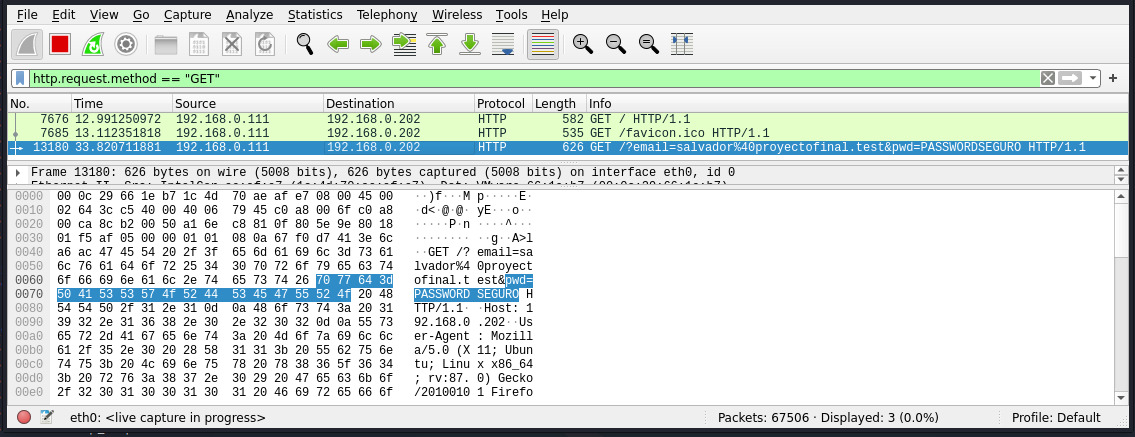
\includegraphics[width=17cm,height=7cm]{paquetes.png}
      \end{center}
      \caption{Paquetes capturados}
      \label{pacCap}
   \end{figure}
\end{center}

Como se puede ver en la figura \ref{pacCap}, Wireshark nos permite filtrar el tráfico, y con el 
simple hecho de decirle que queremos mostrar los requerimientos GET
pudimos dar con el paquete que queríamos, en el request podemos ver
el usuario \texttt{salvador@proyectofinal.test} y la contraseña \texttt{PASSWORD SEGURO}
